%-------------------------
% Resume in Latex
% Template: Sourabh Bajaj
% Author: Lukas Grams
% License : MIT
%------------------------

\documentclass[letterpaper,11pt]{article}

\usepackage{latexsym}
\usepackage[empty]{fullpage}
\usepackage{titlesec}
\usepackage{marvosym}
\usepackage[usenames,dvipsnames]{color}
\usepackage{verbatim}
\usepackage{enumitem}
\usepackage{xcolor}
\usepackage[colorlinks=true, urlcolor=blue, pdfborderstyle={/S/U/W 1},pdfborder=0 0 1, urlbordercolor=blue ]{hyperref}
%\usepackage[hidelinks]{hyperref}
%\usepackage{hyperref}
\usepackage{fancyhdr}
\usepackage{nccfoots}
\usepackage{graphicx}
\graphicspath{{C:/Users/GSYS/Downloads/} }
\usepackage{float}


\pagestyle{fancy}
\fancyhf{} % clear all header and footer fields
\fancyfoot{}
\renewcommand{\headrulewidth}{0pt}
\renewcommand{\footrulewidth}{0pt}

% Adjust margins
\addtolength{\oddsidemargin}{-0.5in}
\addtolength{\evensidemargin}{-0.5in}
\addtolength{\textwidth}{1in}
\addtolength{\topmargin}{-.5in}
\addtolength{\textheight}{1.0in}

\urlstyle{same}

\raggedbottom
\raggedright
\setlength{\tabcolsep}{0in}

% Sections formatting
\titleformat{\section}{
  \vspace{-4pt}\scshape\raggedright\large
}{}{0em}{}[\color{black}\titlerule \vspace{-5pt}]

%-------------------------
% Custom commands
\newcommand{\resumeItem}[2]{
  \item\small{
    \textbf{#1}{: #2 \vspace{-2pt}}
  }
}

\newcommand{\resumeItemWithoutHeadline}[1]{
	\item\small{
		{#1 \vspace{-2pt}}
	}
}

\newcommand{\resumeSubheading}[4]{
  \vspace{-1pt}\item
    \begin{tabular*}{0.97\textwidth}[t]{l@{\extracolsep{\fill}}r}
      \textbf{#1} & #2 \\
      \textit{\small#3} & \textit{\small #4} \\
    \end{tabular*}\vspace{-5pt}
}

\newcommand{\resumeSubItem}[2]{\resumeItem{#1}{#2}\vspace{-4pt}}

\renewcommand{\labelitemii}{$\circ$}

\newcommand{\resumeSubHeadingListStart}{\begin{itemize}[leftmargin=*]}
\newcommand{\resumeSubHeadingListEnd}{\end{itemize}}
\newcommand{\resumeItemListStart}{\begin{itemize}}
\newcommand{\resumeItemListEnd}{\end{itemize}\vspace{-5pt}}

%-------------------------------------------
%%%%%%  CV STARTS HERE  %%%%%%%%%%%%%%%%%%%%%%%%%%%%

\begin{document}

%----------HEADING-----------------
\begin{tabular*}{\textwidth}{l@{\extracolsep{\fill}}r}
	\textbf{\Large Lukas Grams}\\
	{born Sept 20th, 1994 in Düsseldorf, Germany}\\
	{Residence: Rosenheim}\\
	{Tel : +49 151 6519 6156}\\  
	\big[
	\href{https://www.xing.com/profile/Lukas_Grams/cv}{Xing},
	\href{https://github.com/gramsimamsi/}{github},
	\href{https://www.linkedin.com/in/lukas-grams/?locale=de}{linkedin (de)},
	\href{https://www.linkedin.com/in/lukas-grams/?locale=en_US}{linkedin (en)} 
	\big] 
	\vspace*{-2.6cm}	\\
	Mail : \href{mailto:lukas.grams.info@gmail.com}{lukas.grams.info@gmail.com} &
	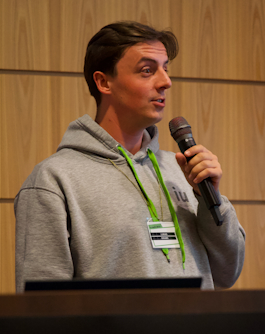
\includegraphics[scale=0.25]{conference.jpeg}\\	
\end{tabular*}

%-----------EXPERIENCE-----------------
\section{Jobs}
  \resumeSubHeadingListStart
  	
	\resumeSubheading
	{Cyber Security Architect}{2021 -- present}
  	{IU Group N.V. - EduTech-Company in the education sector}{Munich}
    \resumeItemListStart
    	\resumeItemWithoutHeadline
    	{Internal stakeholder, ambassador, and advisor for security topics in all business areas and technical teams at operational, conceptual, and leadership levels}
		\resumeItemWithoutHeadline
    	{Presenting and reporting on security topics in workshops, steering committees, and on conferences}
		\resumeItemWithoutHeadline
    	{Building and expanding the 'Cyber Security Services' team and its internal portfolio: \linebreak 
    	SOC (Azure Sentinel, AWS GuardDuty), Incident Response, Security Awareness Programm, \linebreak 
    	Vulnerability Management (Subnet- und Pipeline-Scans, EAM), SDLC (SAST \& DAST), Pentests, Bug Bounties,\linebreak
    	 Audit Response, and Due Diligences for the company and M\&A activities}
	\resumeItemListEnd
 	
	\resumeSubheading
	{Penetration Tester, Security Consultant}{2019 -- 2021}
  	{Atos Information Technology Solutions - Managed Security Service Provider}{Munich}
  	\resumeItemListStart
		\resumeItemWithoutHeadline
       	{Design, planning, and implementing new services: \linebreak Penetration tests \& Security Architecture Consulting for container environments, cloud-hosted and on-premise}
		\resumeItemWithoutHeadline
        {Independent planning and execution of penetration tests, security (architecture) consulting, and security-by-design projects for and with Atos customer}
		\resumeItemWithoutHeadline
		{Focus on Microservices, Container (Clusters), CI/CD Pipelines, Cloud Environments (AWS, Azure), Single-Page Applications, Linux Servers}
	\resumeItemListEnd
	
	\resumeSubheading
	{Junior IT Security Consultant}{2019}
  	{HvS-Consulting - Service provider for security consulting \& assessment}{Garching}
  	\resumeItemListStart
		\resumeItemWithoutHeadline
       	{Operational work in pentesting and social engineering}
       	\resumeItemWithoutHeadline
       	{Supporting ISO27001 certification lead-up}
	\resumeItemListEnd
	
	\resumeSubheading
	{Technical Specialist im Vulnerability Management}{2018}
	{Fujitsu Technology Solutions - Managed Security Service Provider}{Munich}
	\resumeItemListStart
		\resumeItemWithoutHeadline
		{Developing tools, systems, and processes for automating vulnerability management analysis and alerting}
		\resumeItemWithoutHeadline
		{Technologies used: \linebreak
		Docker, Git/GitLab, Ruby, Shell Scripts, Ubuntu, RHEL, Elasticsearch, Logstash, Kibana, Kolide Fleet, Osquery}
	\resumeItemListEnd
	
	
	\resumeSubheading
	{Tutor \& Teaching Assistant (Programming 2, Algorithms \& Data Structures) }{2017 - 2018}
	{Rosenheim University of Applied Sciences, Faculty of Computer Science}{Rosenheim}
	
		
	\resumeSubheading
	{Support Engineer (2nd Level Support)}{2015}
	{Cancom NSG GmbH - IT Service Provider}{Munich}
	
	\resumeSubheading
	{IT Systems Electronics Technician (Printer Service \& Support in Field Service)}{2011 - 2014}
	{Cancom GmbH - IT Service Provider}{Munich}

  \resumeSubHeadingListEnd
 

%-----------EDUCATION----------------
\section{Education}
  \resumeSubHeadingListStart
    \resumeSubheading
   	  {Bachelor of Science in Computer Science}{2015 -- 2019}    
      {Rosenheim University of Applied Sciences,  GPA: 1,6}{Rosenheim}
    \resumeSubheading
      {Vocational Training IT Systems Electronics Technician (IHK)}{2011 -- 2014}
      {Vocational School Munich, GPA: 1.0}{Munich}
  \resumeSubHeadingListEnd

\newpage

%--------Projects------------
\section{Projects}
\resumeSubHeadingListStart

\item{
	\textbf{Private Project Connected Home}{: 	\linebreak 
		Setting up a private Docker setup for AdBlocking, VPN, password manager, and media streaming with Raspberry Pi, HypriotOS, Docker, PiHole, openVPN, KeePass, and OpenPHT}
}
\item{
	\textbf{\href{https://github.com/gramsimamsi/bachelorThesis/blob/master/thesis.pdf}{Kubernetes Attack \& Defense}}{: 	\linebreak 
		Identifying and evaluating attack vectors and defense measures in distributed container environments and deriving prioritized risk management measures based on Docker, Kubernetes, OpenShift, Azure, and RHEL}
}
\item{
	\textbf{\href{https://github.com/gramsimamsi/thirstygames}{Thirstygames}}{: 	\linebreak 
		Tracking, accumulating, and presenting of competitive, team-based consumption of predominantly hop-based beverages. Development of a responsive web app with three people using Angular 7, Material Design, ChartsJs, Express, Docker, and Nginx }
}
\item{
	\textbf{CowTracking}{: 	\linebreak 
		Locating cows using a LoRa-enabled full-stack application consisting of microcontroller, backend, DB, and frontend servers. Presenting the project to both \href{https://www.youtube.com/watch?v=JIbElz2qEes}{large-scale audiences} as well as \href{https://www.rfo.de/mediathek/video/digitalisierungsmesse-an-der-hochschule-rosenheim/}{press} }
}
\resumeItemListEnd
%-------------------------------------------

%--------SKILLS------------
\section{Miscellaneous}
\resumeSubHeadingListStart
\item{
	\textbf{Certificates}{: 
		\resumeItemListStart
		\resumeItemWithoutHeadline
		{GPEN (GIAC Certified Penetration Tester)}
		\resumeItemWithoutHeadline
		{In Progress: AWS Certified Security – Specialty}
		\resumeItemListEnd
}}
\item{
	\textbf{Languages}{: 	
		\resumeItemListStart
		\resumeItemWithoutHeadline
		{English: Fluent in presentation and negotiation, both written and spoken}
		\resumeItemWithoutHeadline
		{German: Native}
		\resumeItemListEnd
}}
\resumeSubHeadingListEnd
%-----------------------------

%-----------VOLUNTEERING-----------------
\section{Volunteering}
  \resumeSubHeadingListStart  
  	
  	\resumeSubheading
  	{GIAC Advisory Board Member}{2020 - present}
  	{Global Information Assurance Certification}{}
  	\resumeItemListStart
  		\resumeItemWithoutHeadline
  		{Occasional input on the direction and design of InfoSec training.}
  	\resumeItemListEnd
  	
  	\resumeSubheading
  	{OWASP Member}{2018 - present}
  	{Open Web Application Security Project}{}
  	\resumeItemListStart
  		\resumeItemWithoutHeadline
  		{Minor contributions to the OWASP Docker Top 10}
  		\resumeItemWithoutHeadline
  		{Participant in Munich OWASP meetups}
  	\resumeItemListEnd
  	  
	\resumeSubheading
	{Student year representative and active Student Council Member}{2015 - 2019}
	{Hochschule Rosenheim, Fakultät Informatik}{Rosenheim}
	\resumeItemListStart
		\resumeItemWithoutHeadline
		{Bilateral representation of students and professors}
		\resumeItemWithoutHeadline
		{Organization of informational events, parties, and other happenings}
	\resumeItemListEnd
	
	\resumeSubheading
	{Training future youth counselors}{2015 - 2017}
	{Jugendwerk Rosenheim}{Rosenheim}
	\resumeItemListStart
		\resumeItemWithoutHeadline
		{Training and further education of current and prospective youth counselors}
		\resumeItemWithoutHeadline
		{Conceptual steering and budget planning of the non-profit org}
		\resumeItemWithoutHeadline
		{Planning and conducting trainings, one- and multi-day-events}
	\resumeItemListEnd
	
  \resumeSubHeadingListEnd
%-----------------------------

\raggedleft 
\tiny{This resume is written in LaTeX. The source file can be found in my GitHub \href{https://github.com/gramsimamsi/resume/blob/master/lukas_grams_resume.tex}{github repo}.}
\end{document}
